\chapter{结果部分}
\label{chap:result}

\section{机器学习方法结果}
\label{sec:fourpone}

\subsection{粒子重建结果}
\label{sec:fourponepone}

以$\tau^+ \to \pi^+ + \bar{\nu}_{\tau} $过程为例，利用OmniLearn生成模型可得中微子动量信息(Recon)，并与蒙特卡洛模拟产生的重建级数据(Truth)相比较，结果如下图所示。
\begin{figure}[htb]
  \centering
  \subfloat[横向动量]{
    \label{sfig:nu1}
    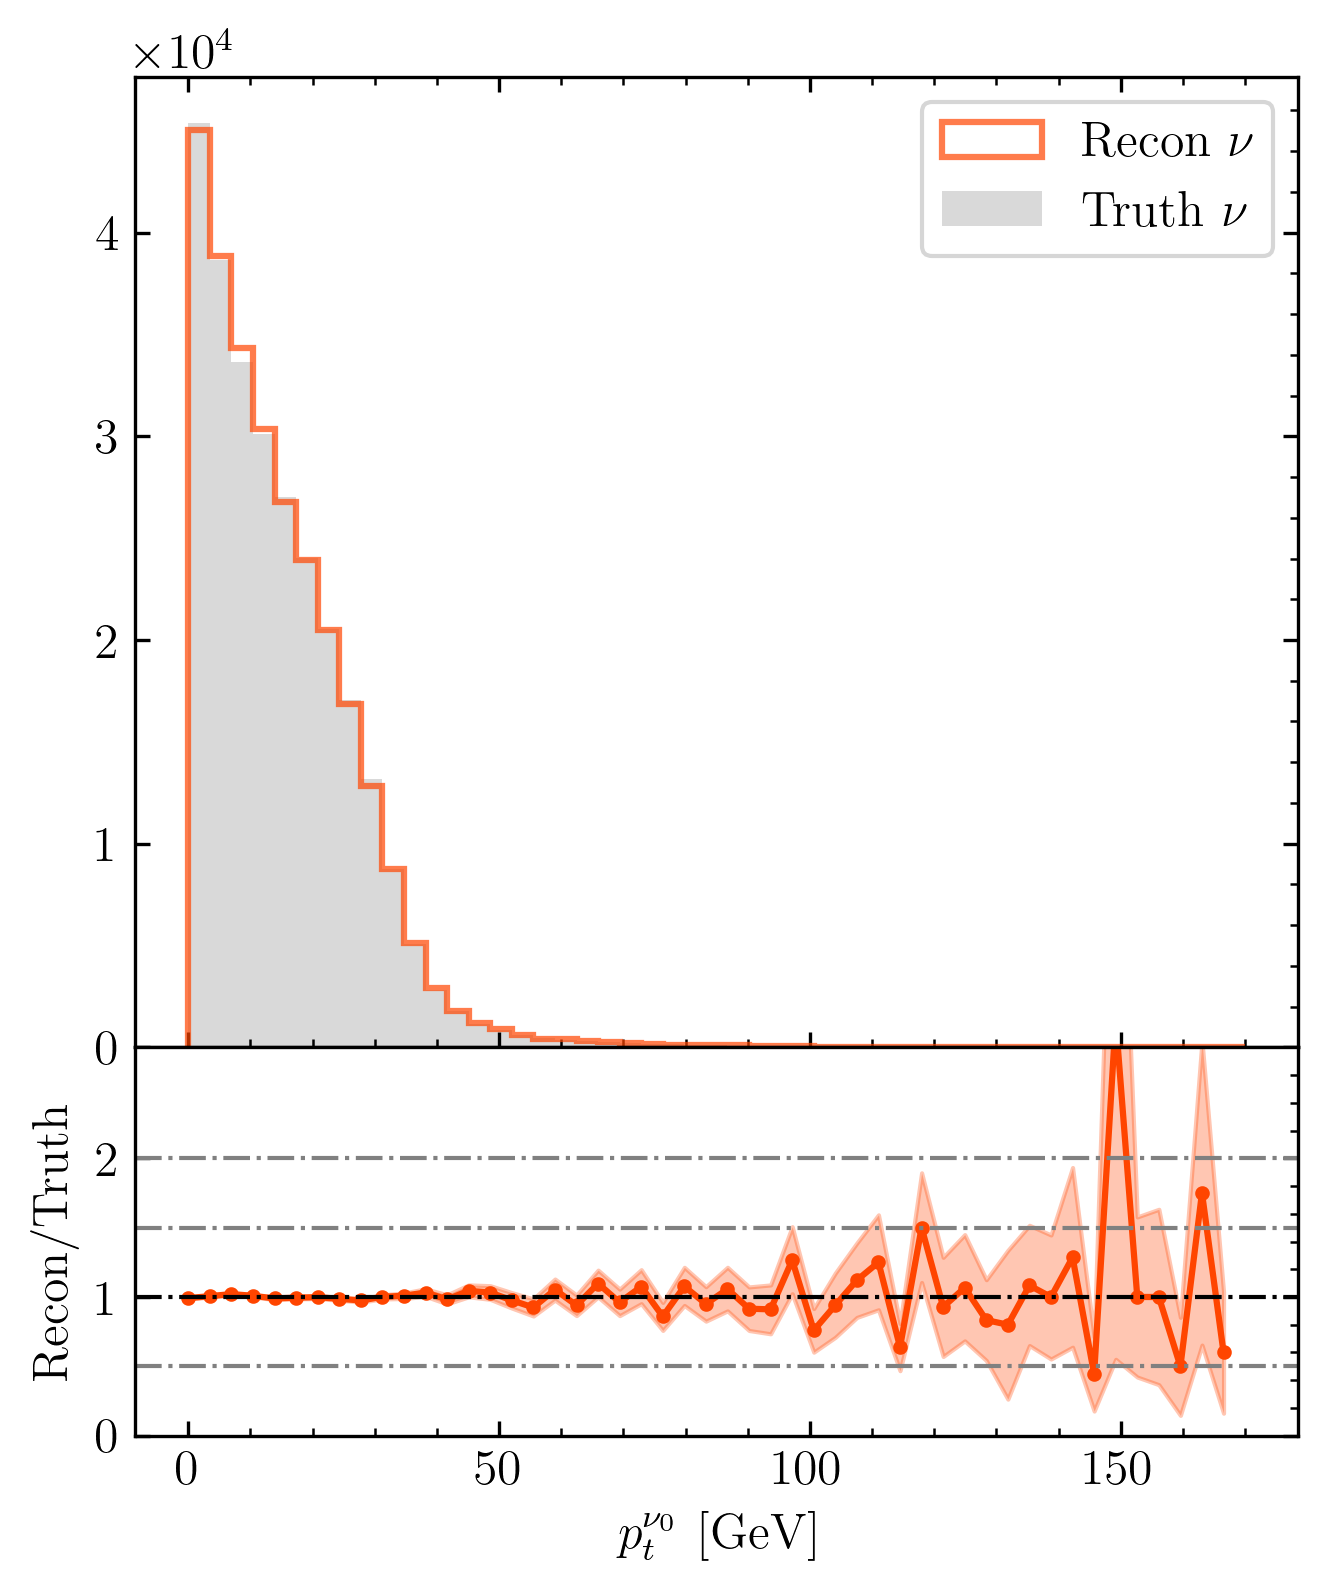
\includegraphics[height=5.85cm]{figures/nu1}}
  \subfloat[赝快度]{
    \label{sfig:nu2}
    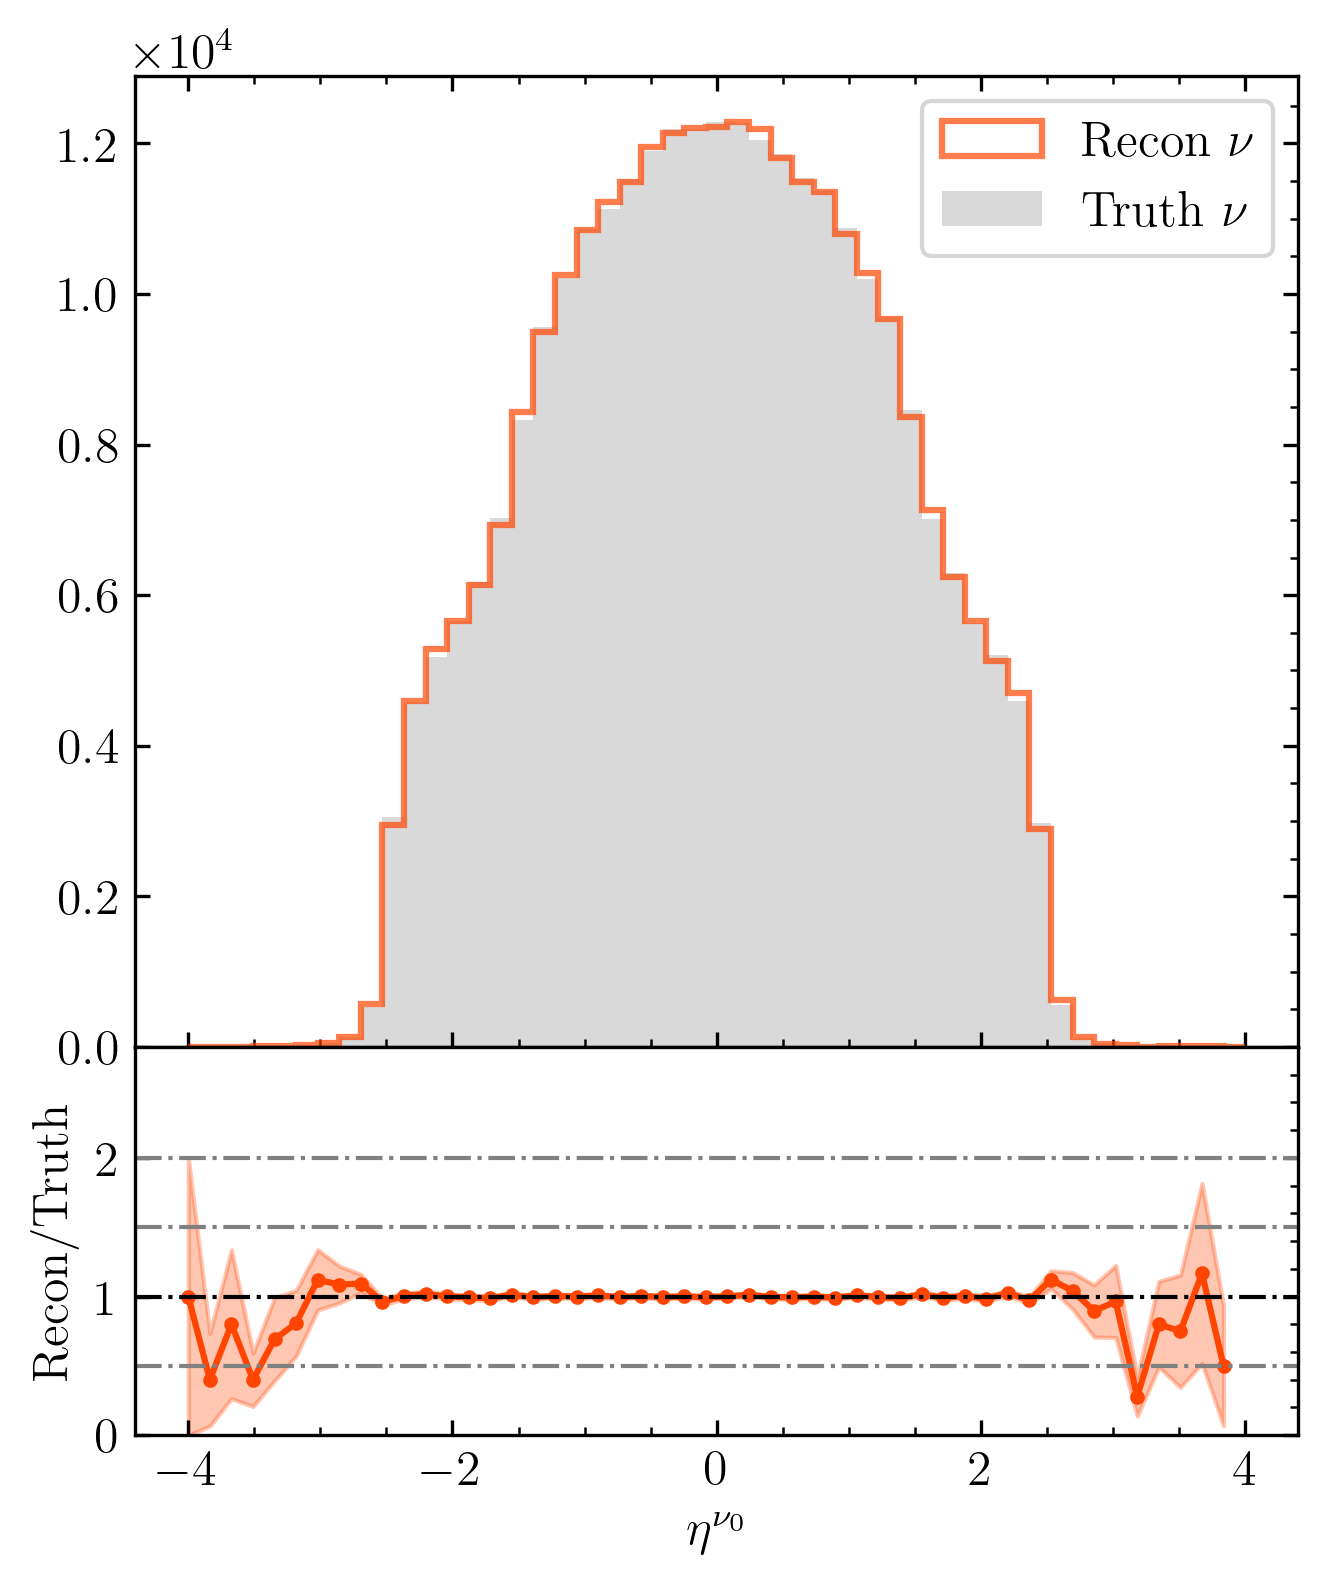
\includegraphics[height=5.80cm]{figures/nu2}}
  \subfloat[方位角]{
    \label{sfig:nu3}
    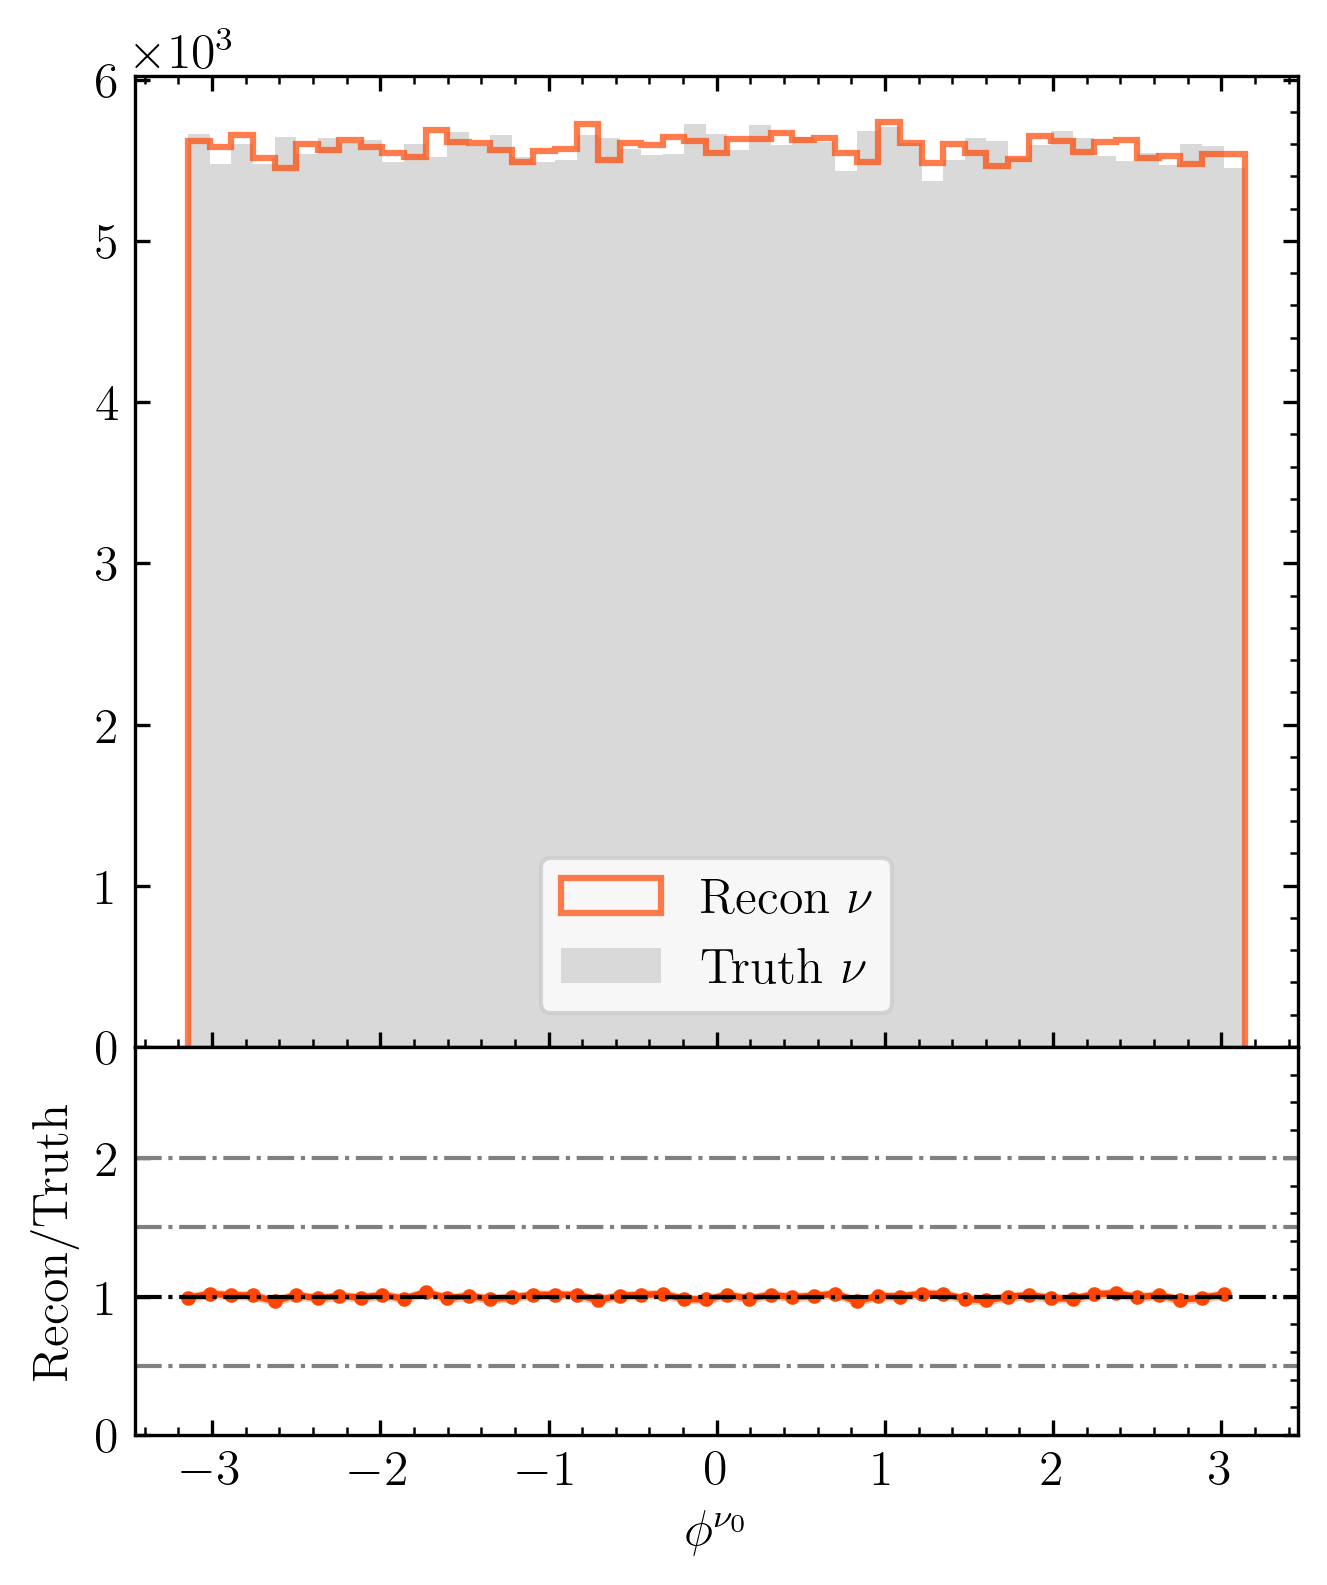
\includegraphics[height=5.78cm]{figures/nu3}}
  \caption{中微子动量信息}
  \label{fig:neutrino}
\end{figure}

图4-1上方的直方图统计所有事件中中微子横向动量、赝快度和方位角的分布；下方的曲线对应各动量信息的生成数据与蒙特卡洛模拟数据二者的事件分布之比，其中浅色阴影部分表示$\pm 1\sigma$ 范围内的泊松误差。

由图可知，对于中微子动量，两个分布吻合得较好，体现出该机器学习方法强大的特征提取和生成能力。

利用动量守恒可进一步得到$\tau$ 子的四动量信息，其结果可见图4-2。
\begin{figure}[htb]
  \centering
  \subfloat[横向动量]{
    \label{sfig:tau1}
    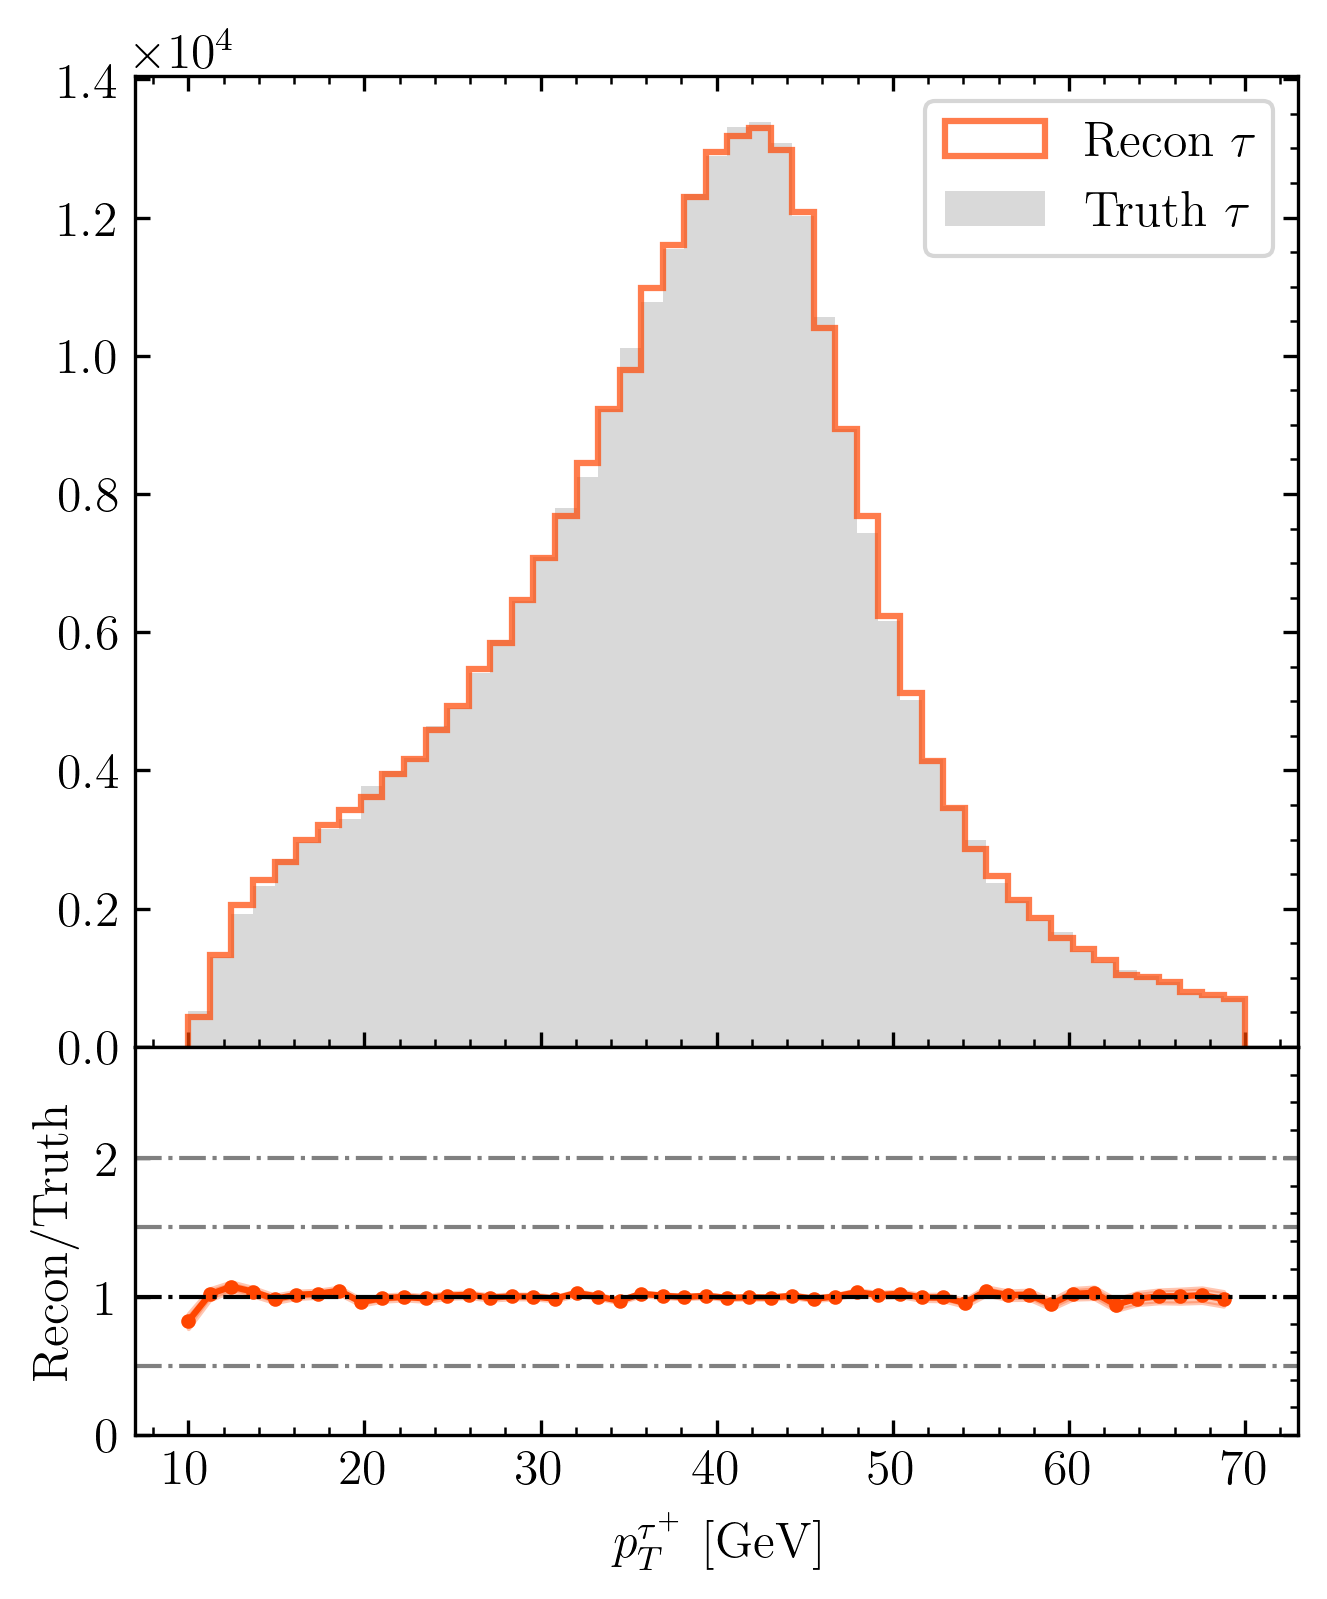
\includegraphics[height=5.88cm]{figures/tau1}}
  \subfloat[赝快度]{
    \label{sfig:tau2}
    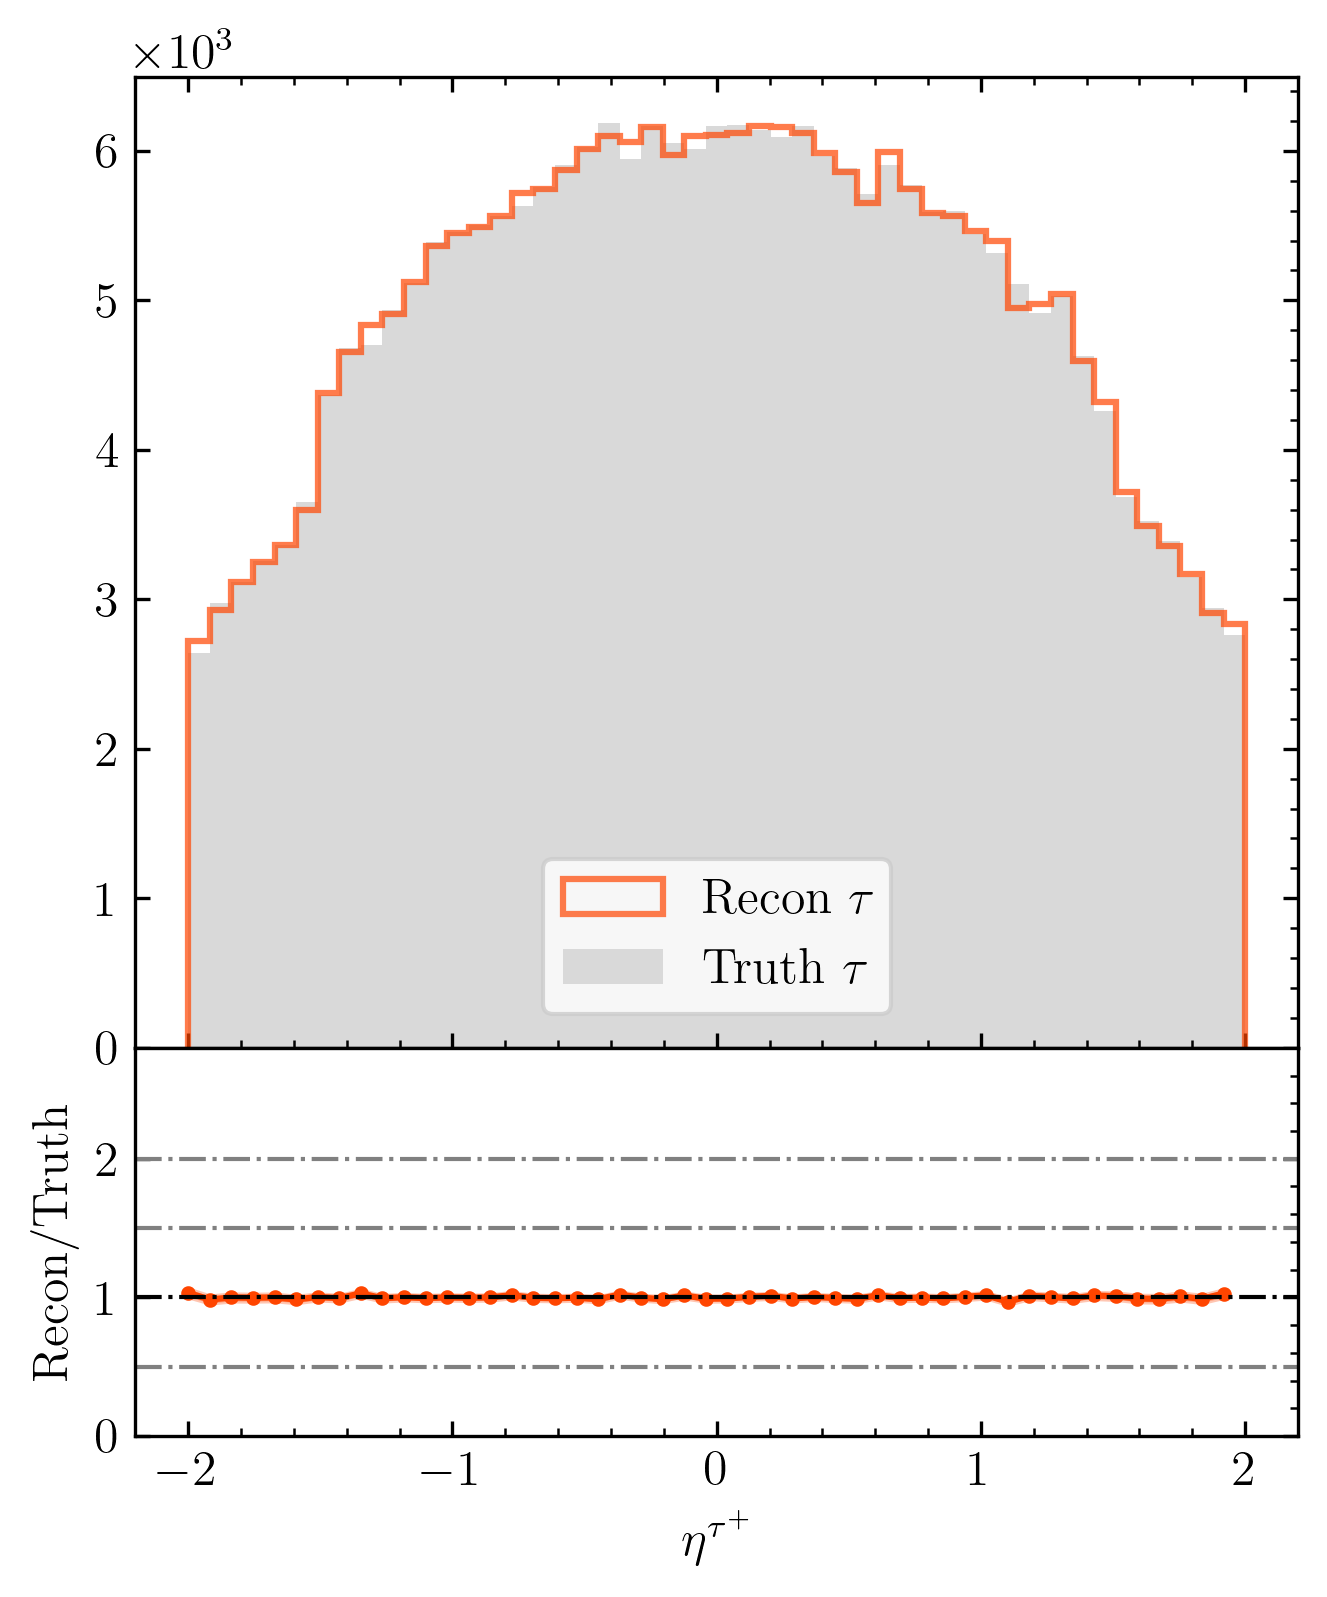
\includegraphics[height=5.87cm]{figures/tau2}}
  \subfloat[方位角]{
    \label{sfig:tau3}
    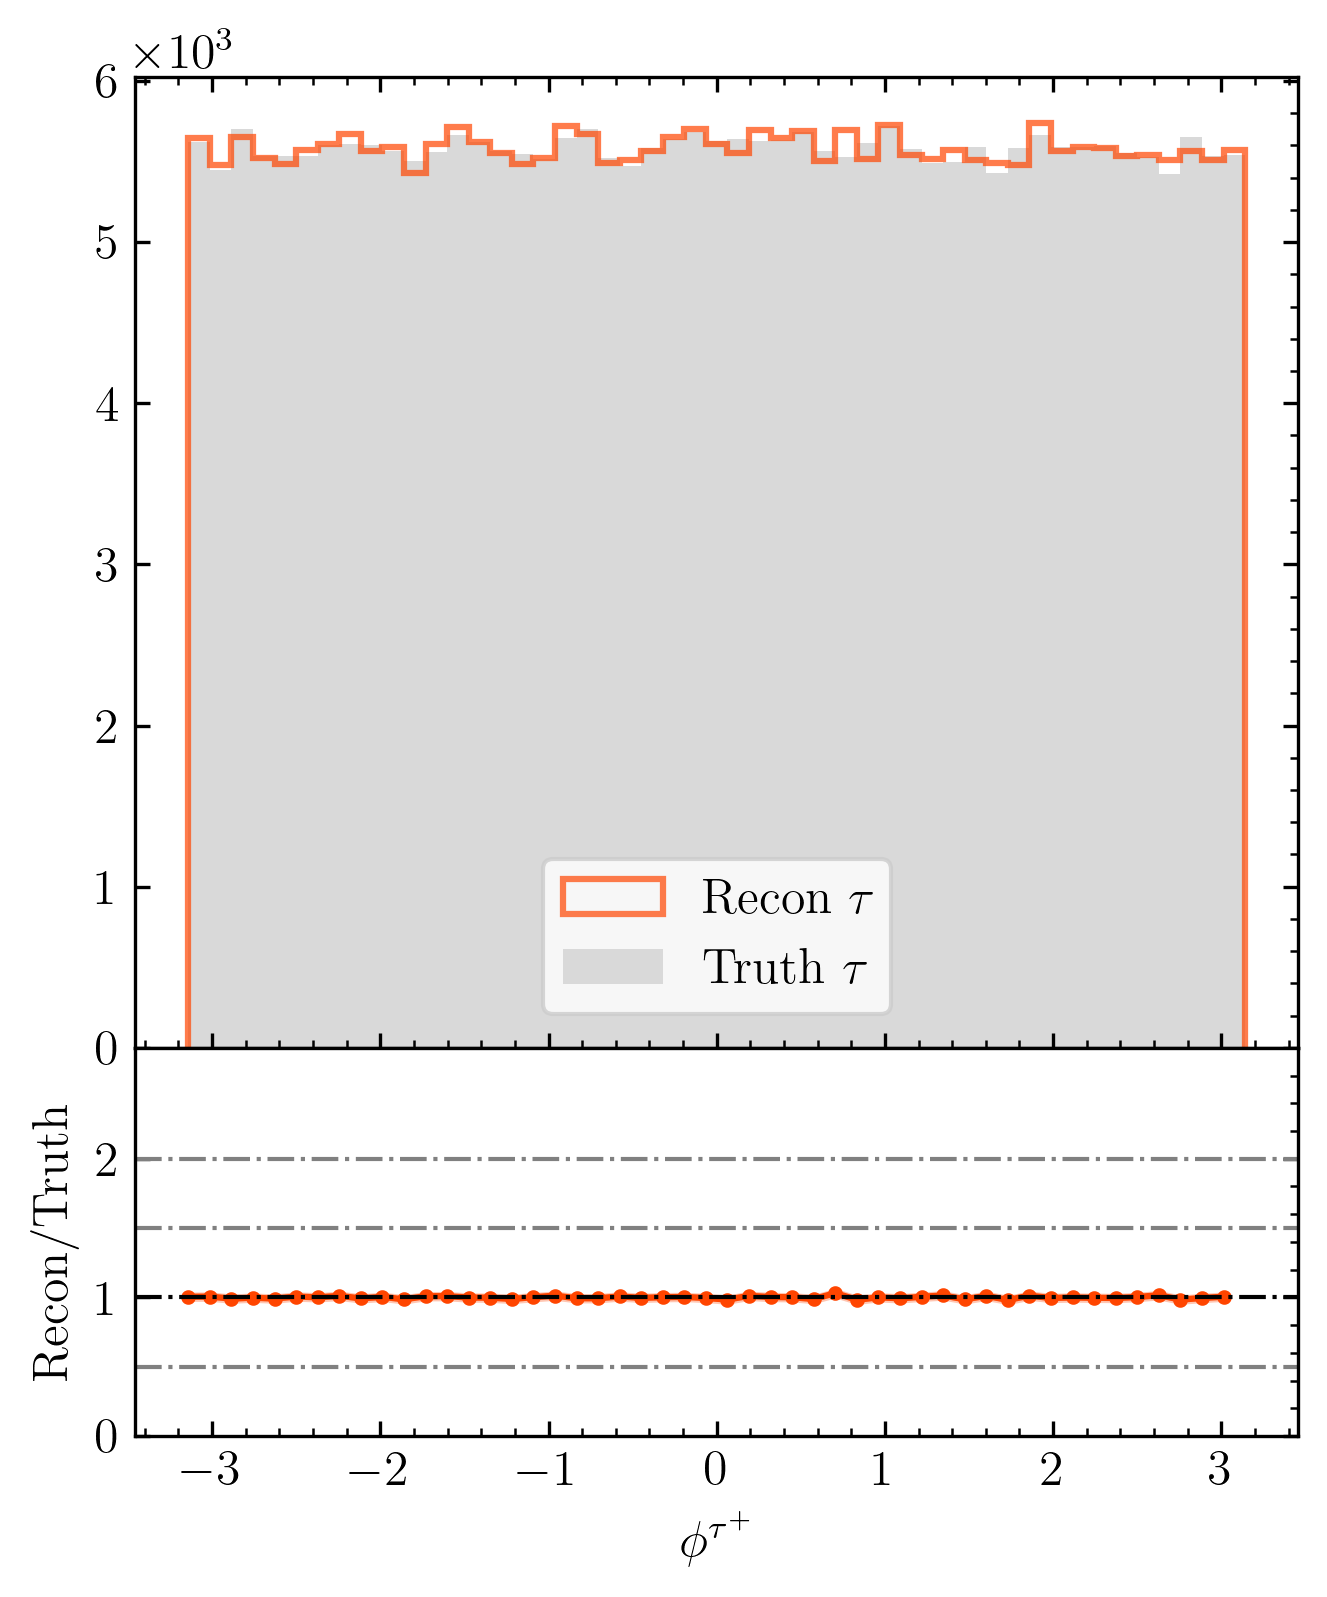
\includegraphics[height=5.91cm]{figures/tau3}}\hspace{4em}
  \subfloat[不变质量]{
    \label{sfig:tau4}
    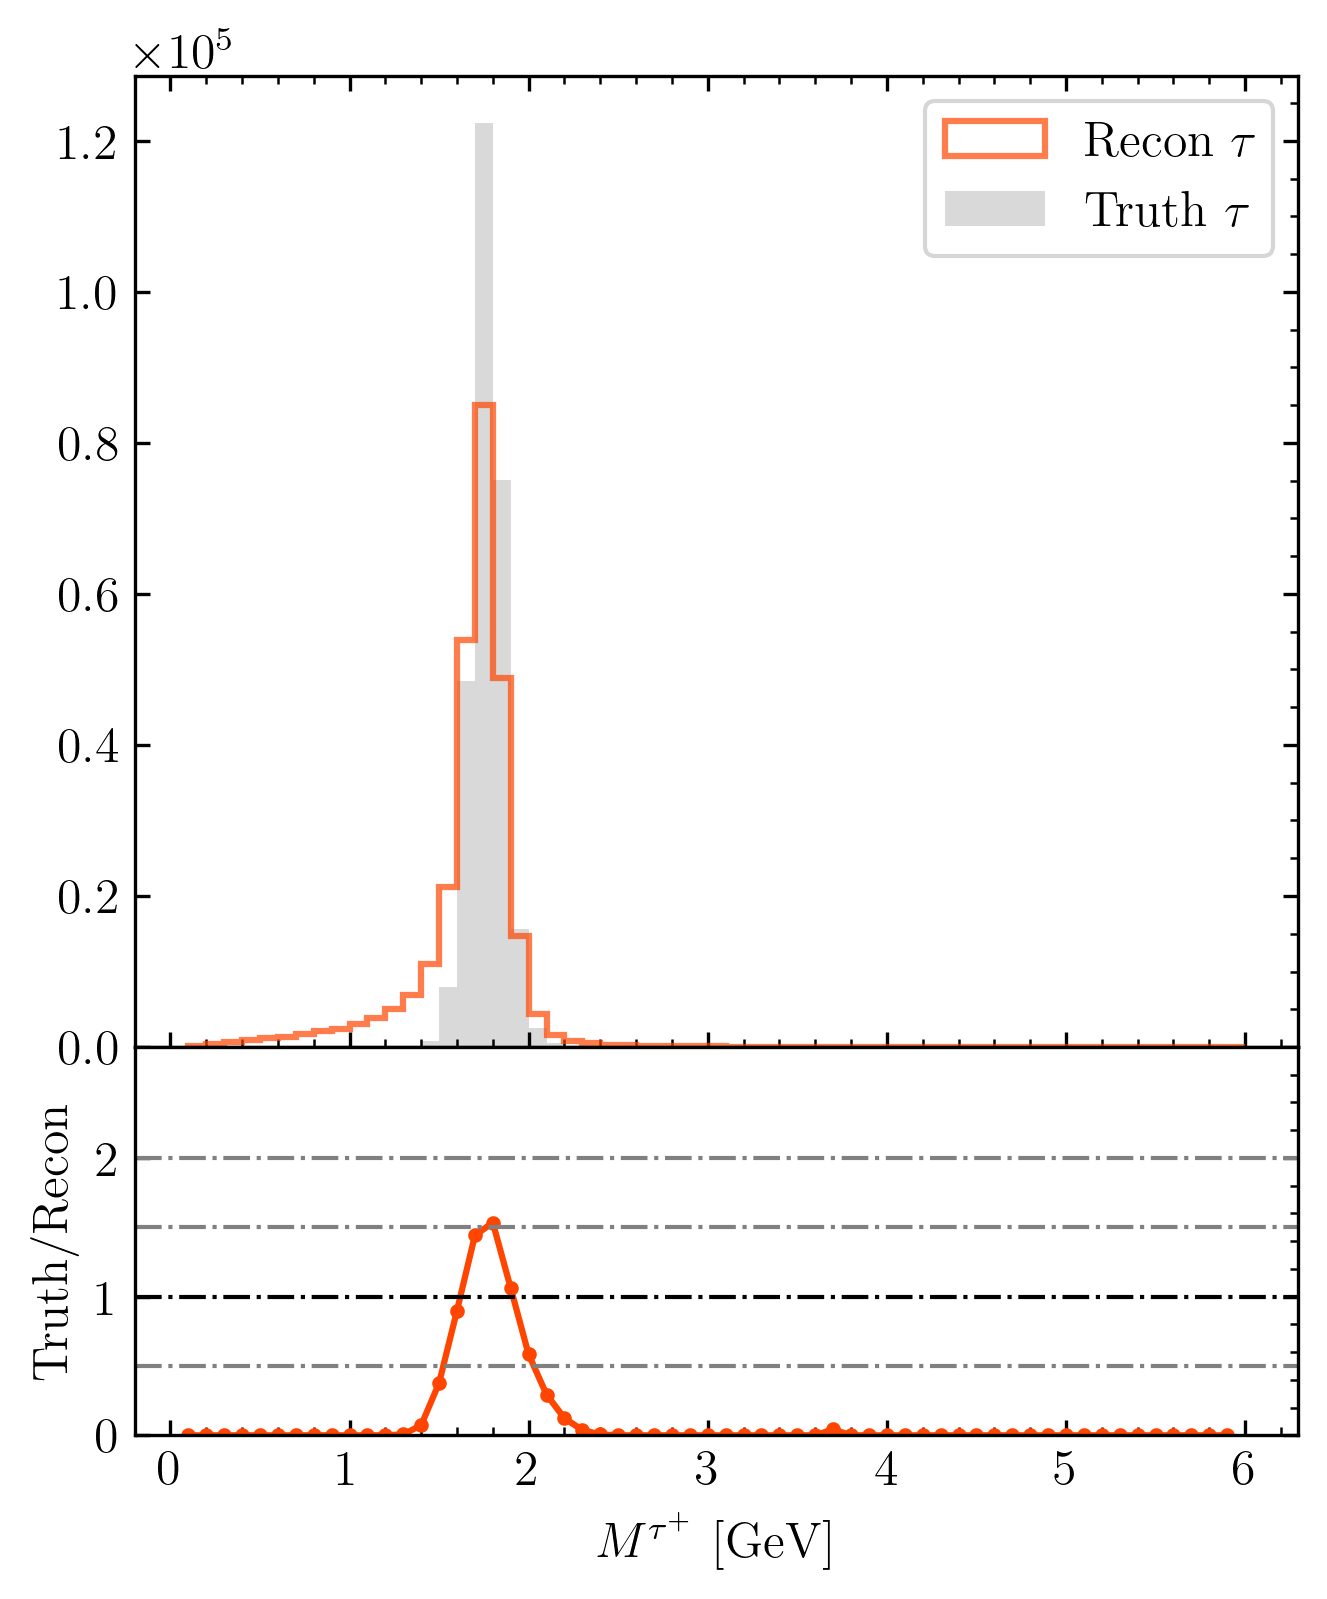
\includegraphics[height=5.91cm]{figures/tau4}}
  \caption{$\tau$子四动量信息}
  \label{fig:tau}
\end{figure}

图4-2中$\tau$ 子的动量信息保持有较高的吻合度，对于其不变质量，生成模型得到的结果在\textit{M}=1.777 GeV附近存在一定的展宽，但这实际上仍然是非常杰出的表现。
此外，还可以得到$\tau^+ \tau^-$对的质量和，该结果将在4.2.2节中与MMC方法比较时一并展现。

\subsection{$\cos  \theta^{\mathcal{A}} \cos  \theta^{\mathcal{B}}$分布计算结果}
\label{sec:fourponeptwo}
按照2.3.3节步骤，可获得$\cos  \theta^{\mathcal{A}} \cos  \theta^{\mathcal{B}}$分布，其中$\mathcal{A}$对应$\tau^+$ ，$\mathcal{B}$对应$\tau^-$ ，与模拟数据(Reconstructed)所得相比较，其结果如图4-3所示。
\begin{figure}[htb]
  \centering
  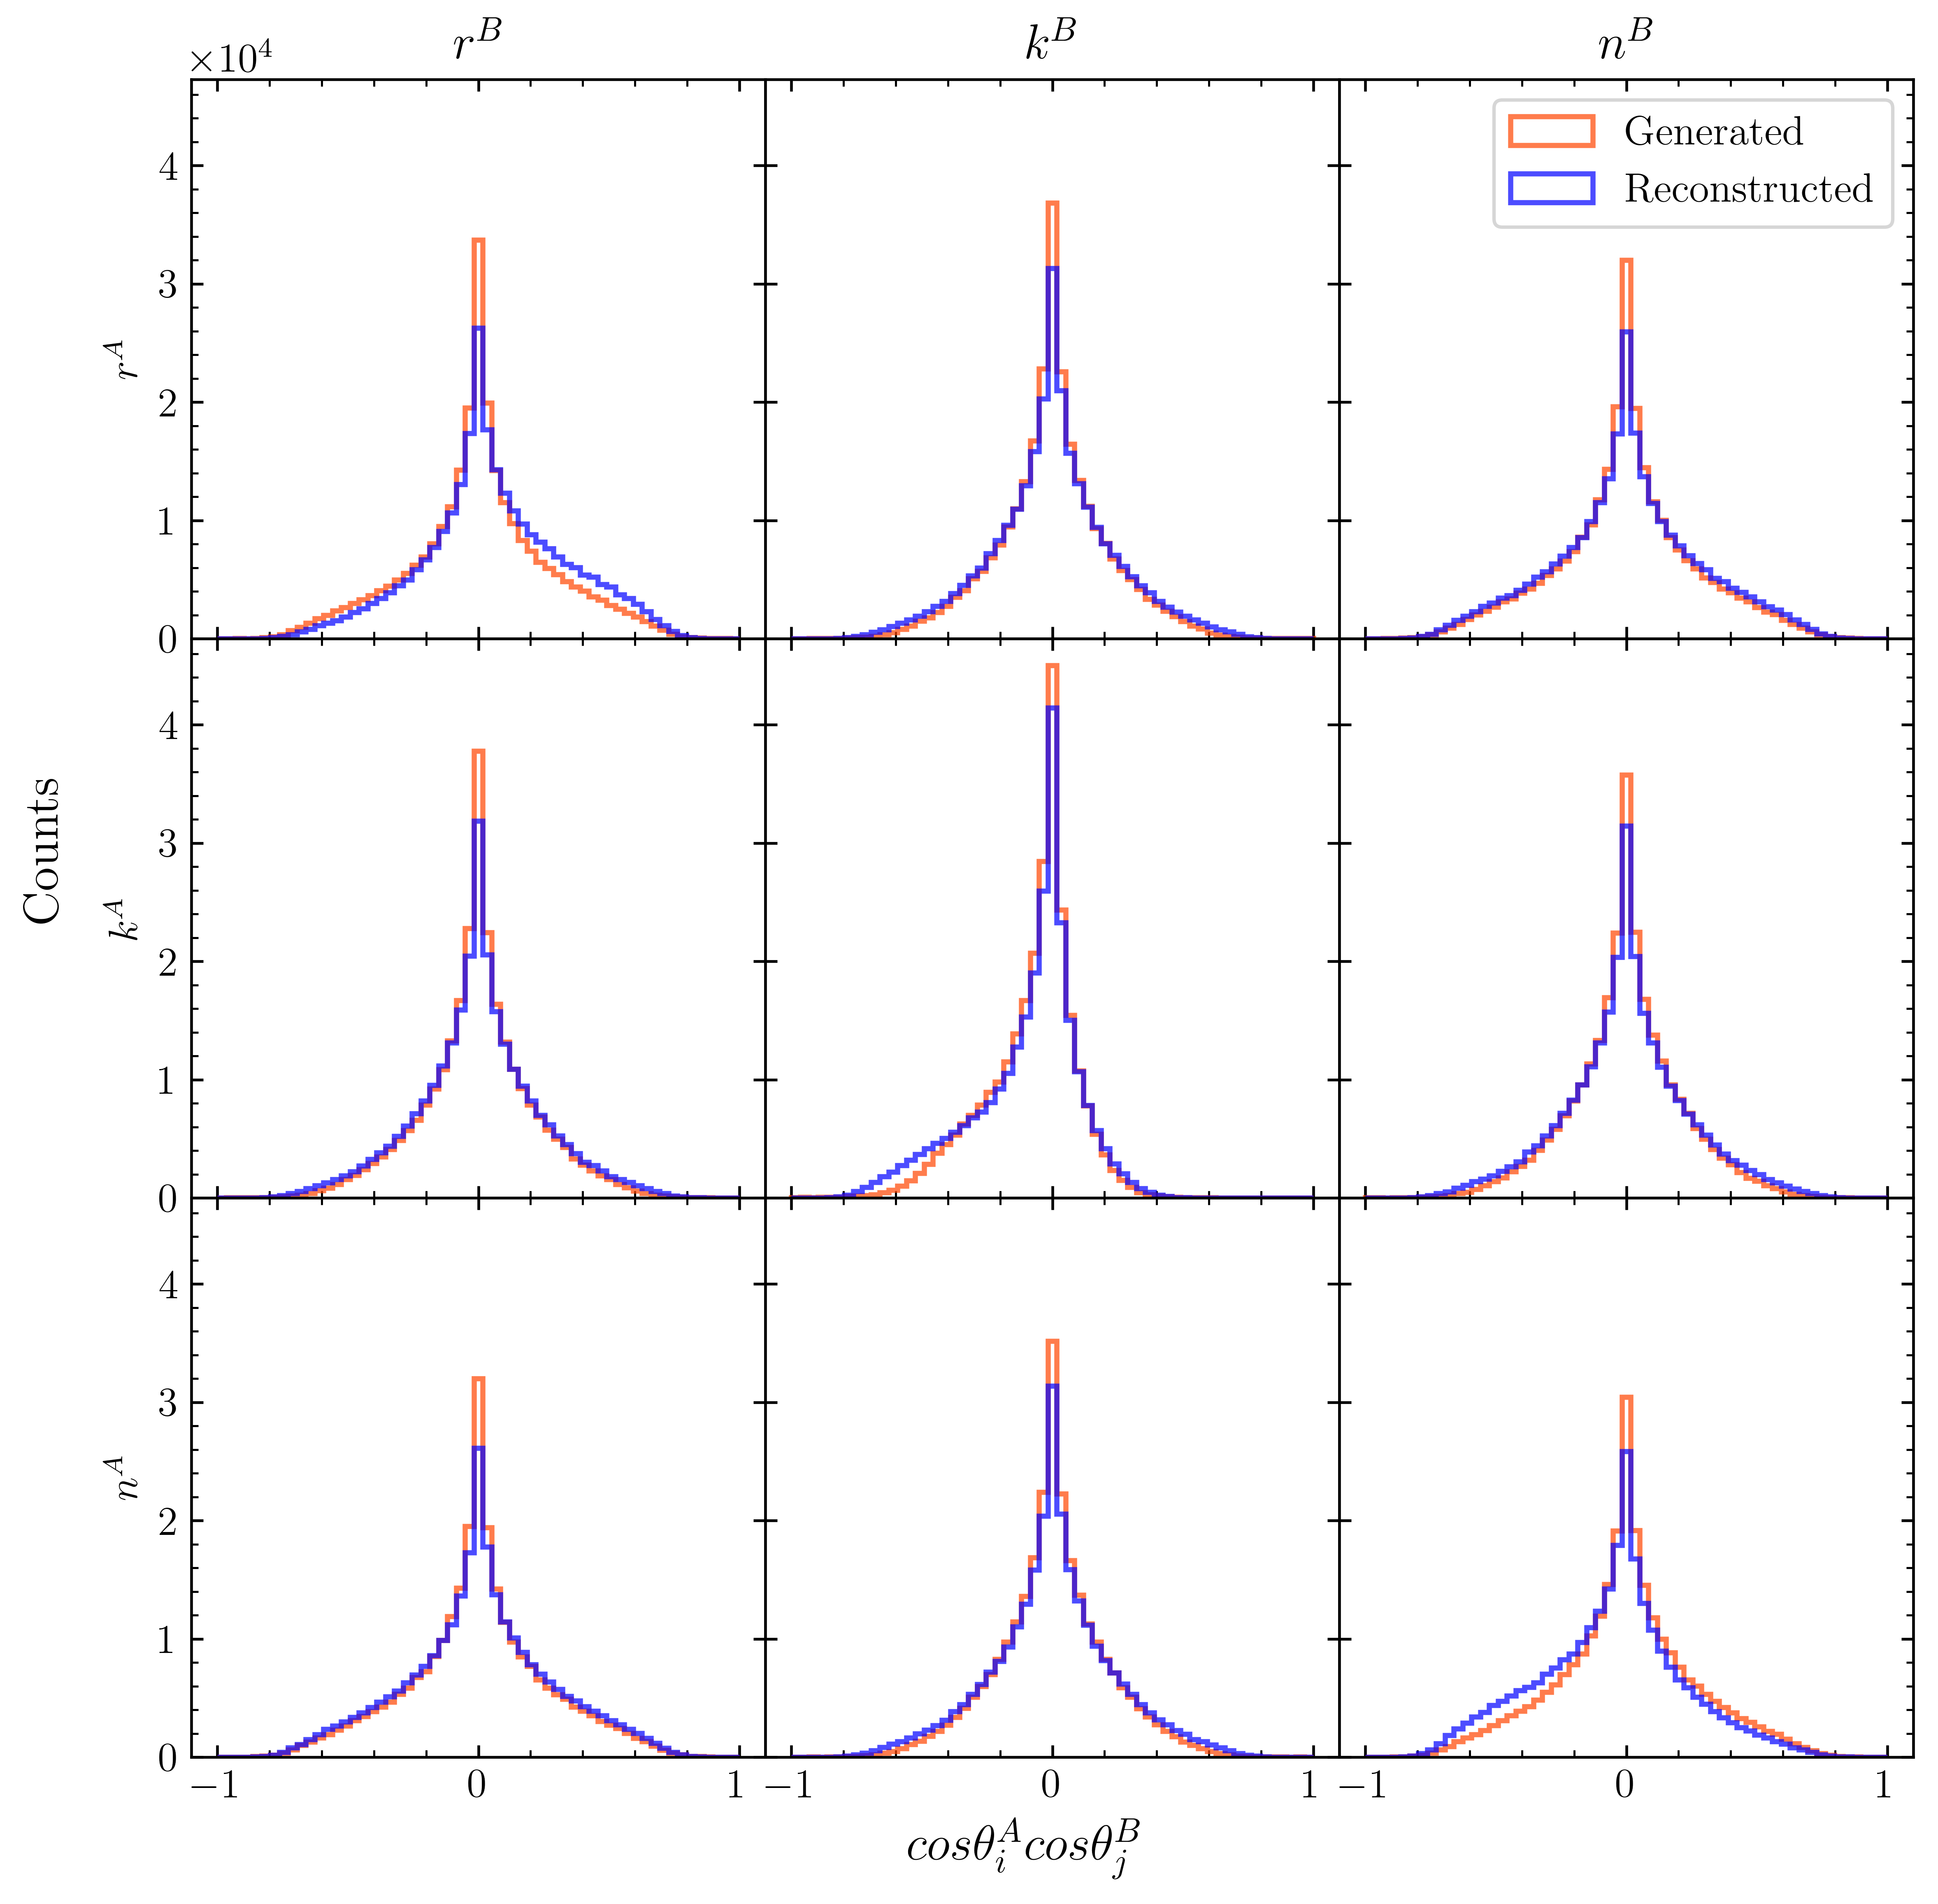
\includegraphics[height=10.0cm]{figures/cos}
  \caption{$\cos  \theta^{\mathcal{A}} \cos  \theta^{\mathcal{B}}$分布}
  \label{fig:coscos}
\end{figure}

按(2.17)式定义，$\theta_{i}^{\mathcal{A}}$ ($\theta_{j}^{\mathcal{B}}$ )是在粒子$\tau^+$(粒子$\tau^-$)的静止参考系下，衰变产物$\pi^+ $($\pi^-$)的动量方向与第$i$($j$)个坐标轴之间的夹角，其中坐标轴分别对应螺旋度基中的$\hat{r}$，$ \hat{k}$，$ \hat{n}$。图4-3的所有子图直观展现各变量的不对称度，并可借此计算自旋关联矩阵的各矩阵元。

此外，不对称度更明显体现在对角元上，对角元细节可见图4-4。
\begin{figure}[htb]
  \centering
  \subfloat[$n$轴]{
    \label{sfig:cosn}
    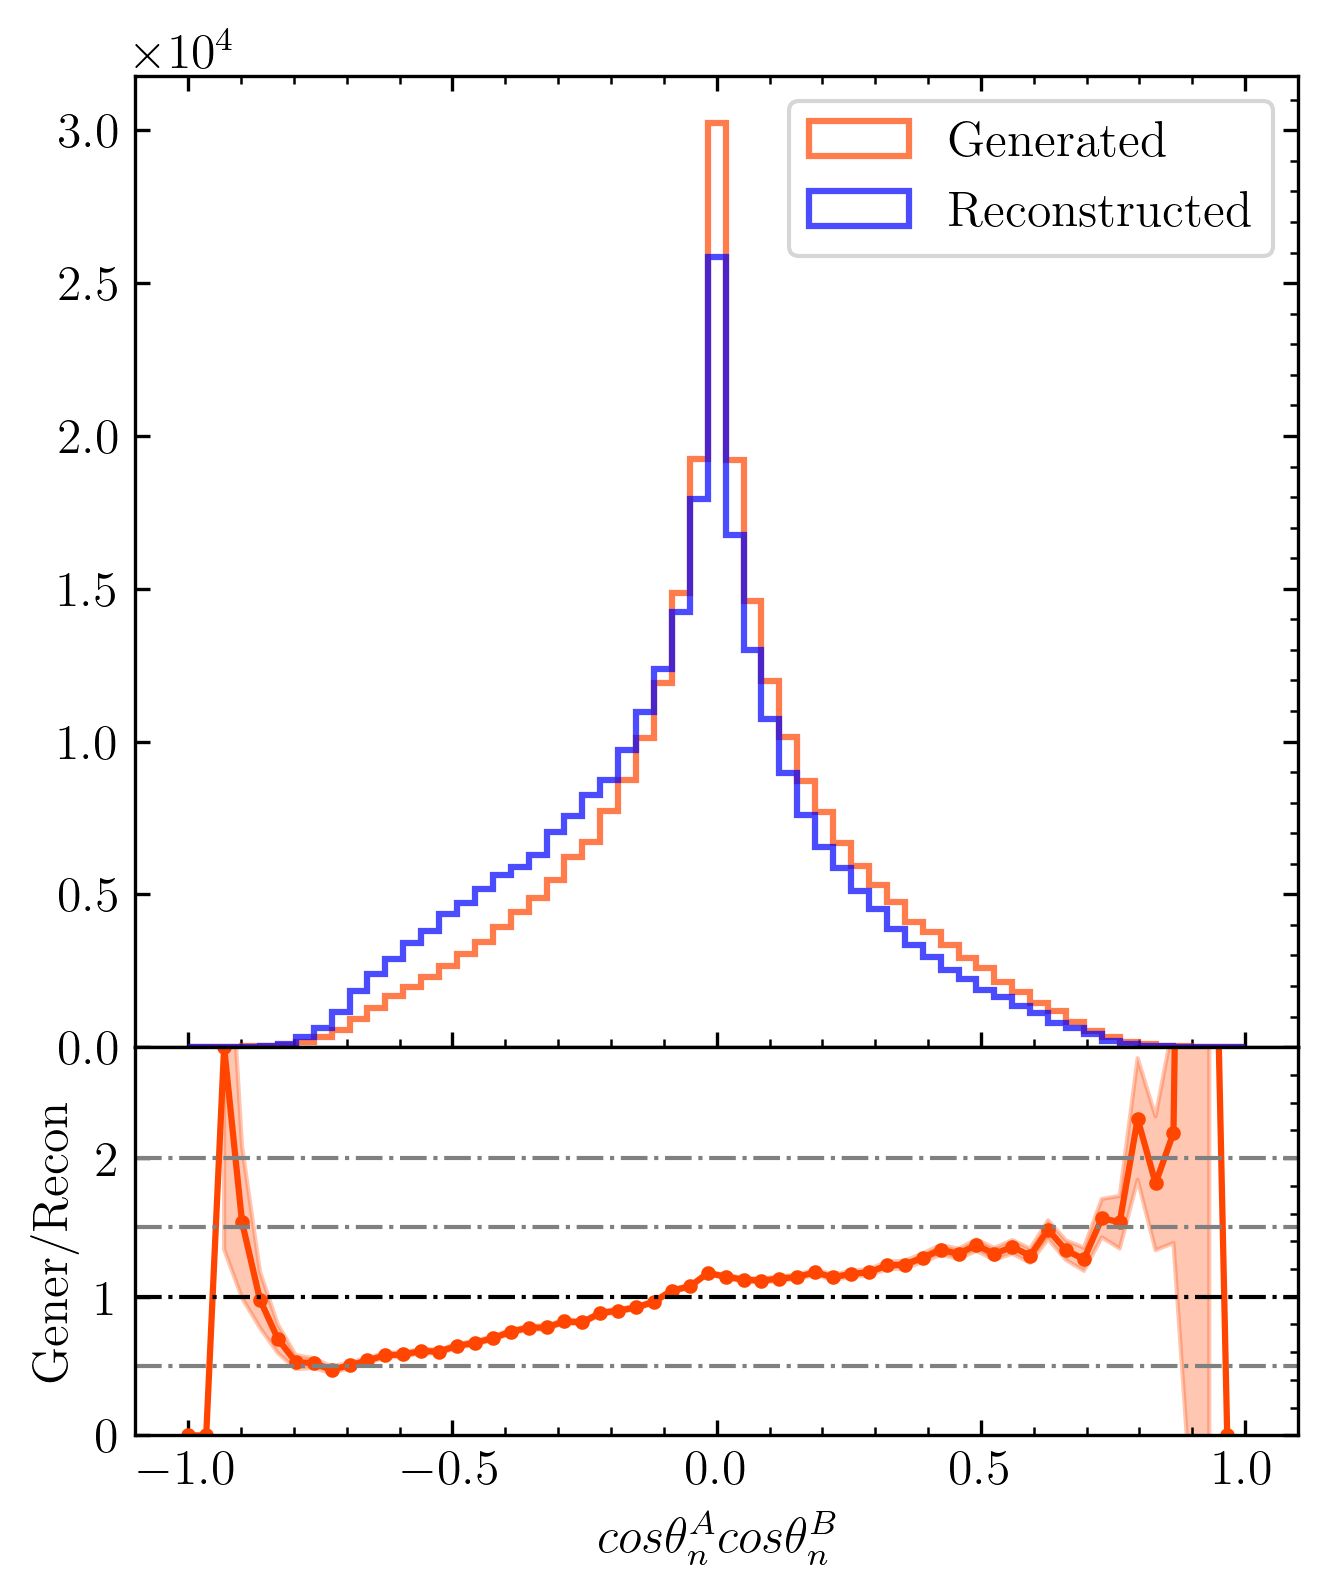
\includegraphics[height=5.86cm]{figures/cosn}}
  \subfloat[$k$轴]{
    \label{sfig:cosk}
    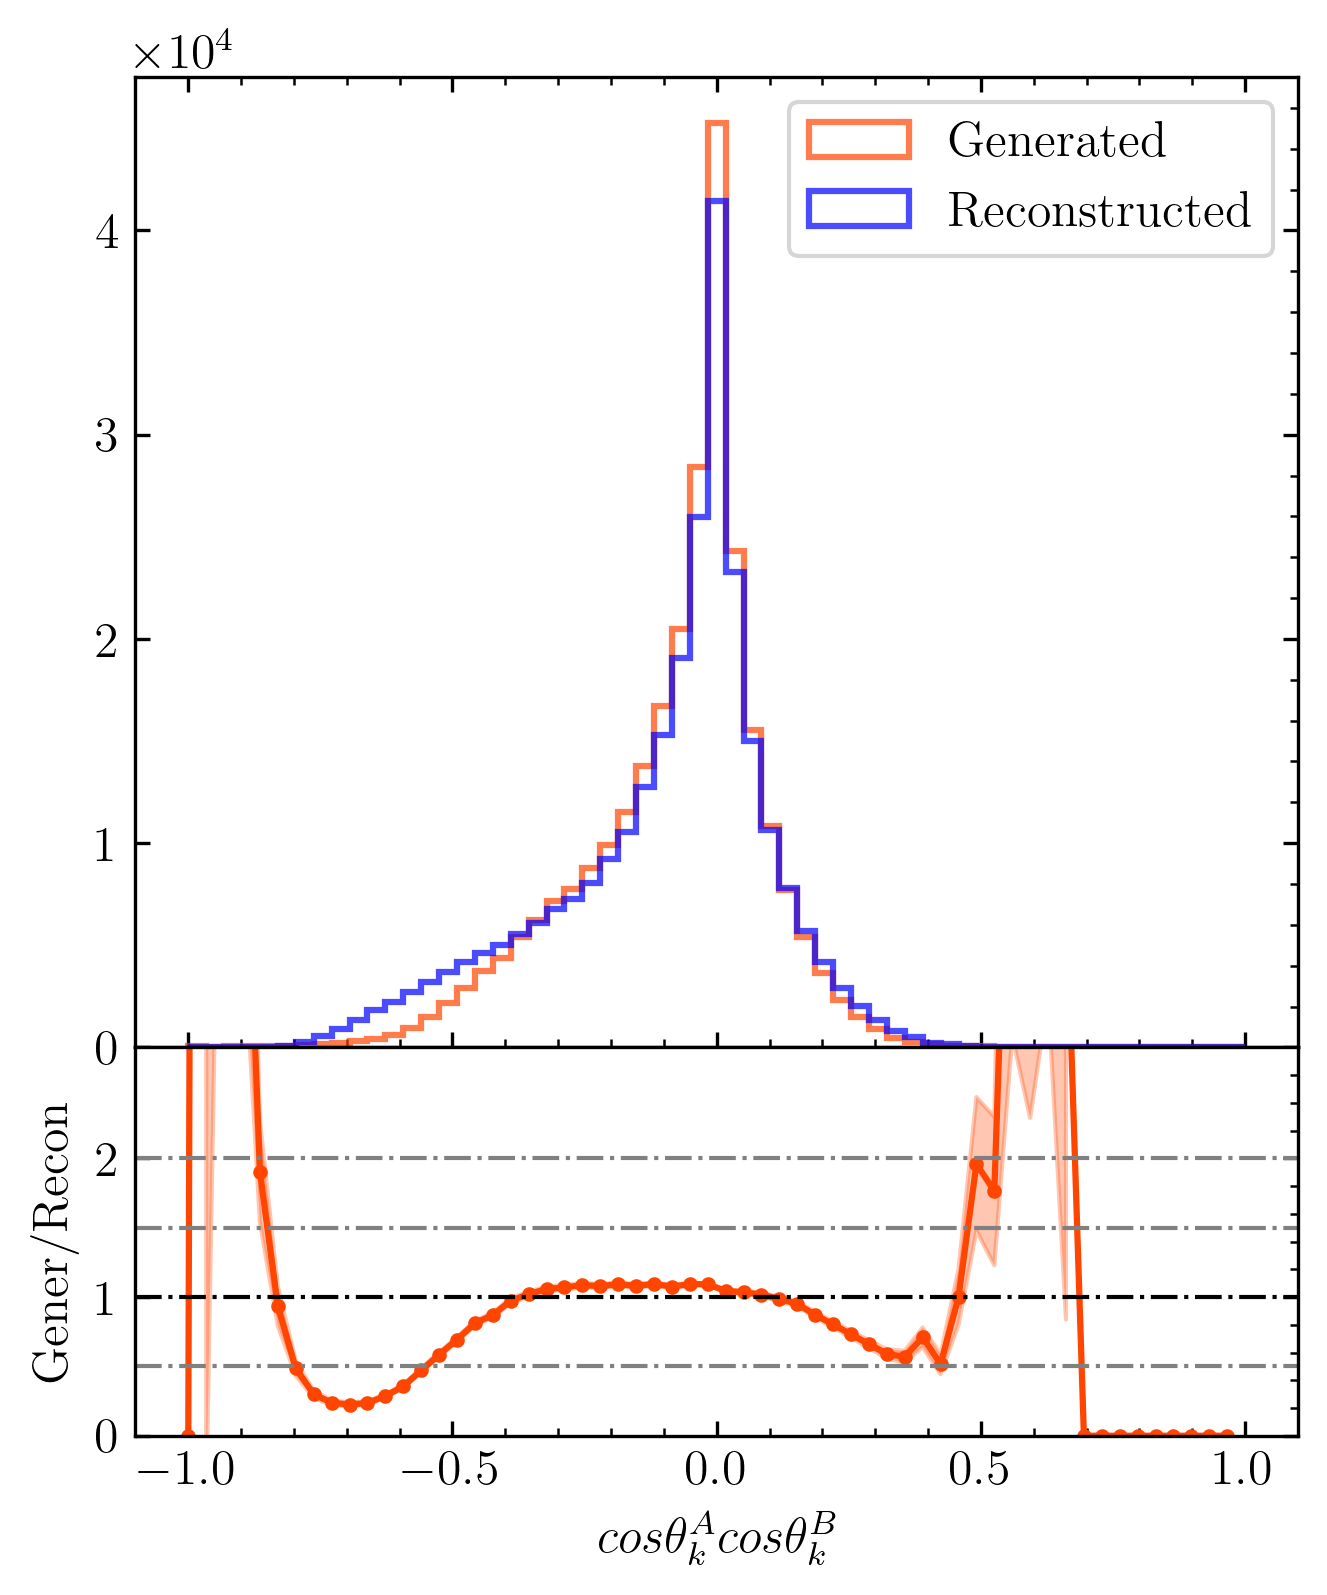
\includegraphics[height=5.83cm]{figures/cosk}}
  \subfloat[$r$轴]{
    \label{sfig:cosr}
    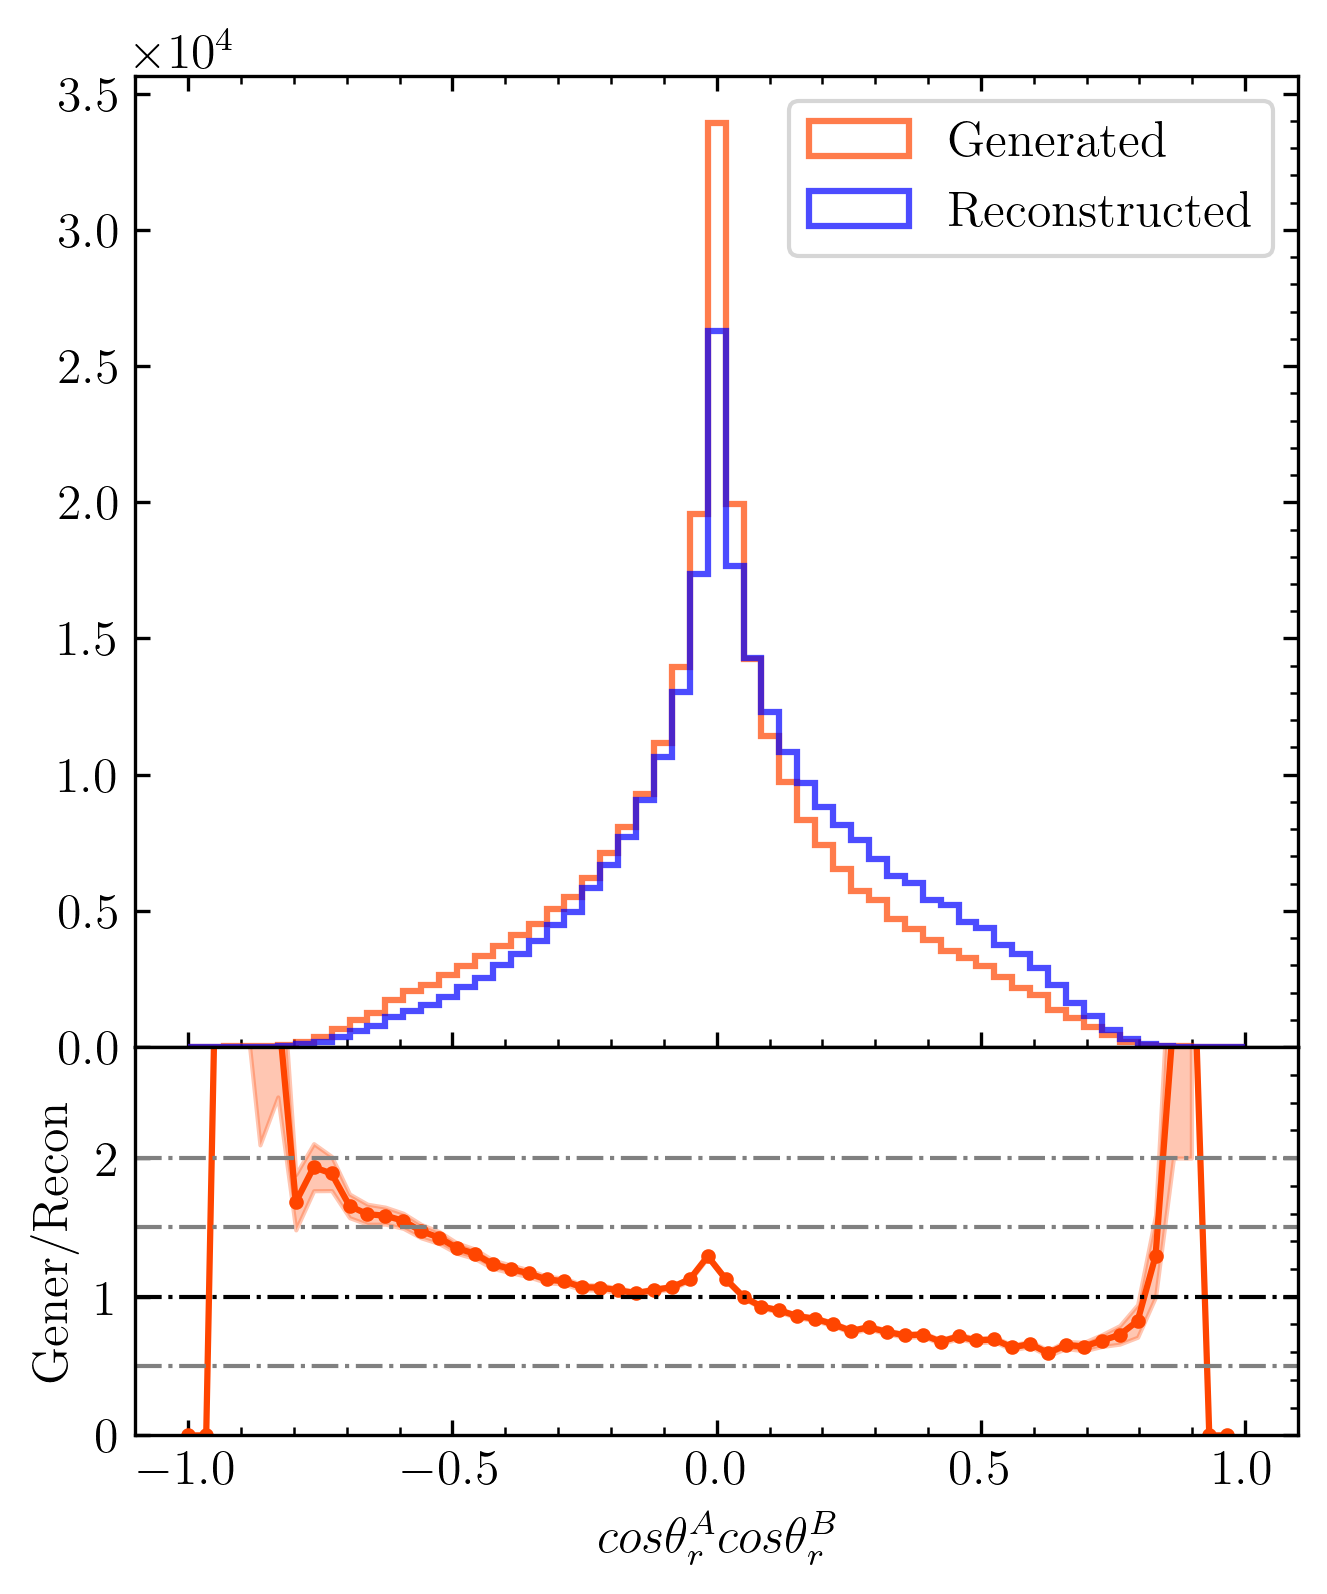
\includegraphics[height=5.82cm]{figures/cosr}}
  \caption{对角元分布比较}
  \label{fig:diag}
\end{figure}

由图4-4可知，对于$n$轴和$k$轴，余弦乘积分布中值小于0的事件数更多；对于$r$轴，其值大于0更有可能。比较机器学习结果和模拟数据结果，可以发现生成数据的余弦乘积分布在变量中心处往往具有更多的事件数，其不对称度也相比原始数据有一小段偏离，但整体仍符合得较好。

\subsection{自旋关联矩阵与纠缠判据计算结果}
\label{sec:fourponepthree}
利用(2.21)式，分别计算两个数据集的自旋关联矩阵$C_{ij}$，并考虑生成模型每次运行结果的不一致性，对该过程重复运行300次以取平均值和标准差，最终结果如下表所示：
\begin{table}[htbp]
  \centering
  \caption{自旋关联矩阵}
  \label{tab:spincorre}
  \renewcommand{\arraystretch}{1.3}
  \begin{tabular}{c|c c c }
    \toprule[1.5pt]
    $C_{ij}^{\text{MC}}$ & $r$ & $k$ & $n$ \\
    \midrule[1pt]
    $r$ & -0.6066 & 0.0012& -0.0298 \\
    $k$ & 0.0080 & 1.2178 &-0.0047 \\
    $n$ & -0.0364 & -0.0046 &0.6343 \\
    \midrule[1.5pt]
    $C_{ij}^{\text{ML}}$ & $r$ & $k$ & $n$ \\
    \midrule[1pt]
    $r$ & -0.0760$\pm$0.0072 & 0.0128$\pm$0.0070& -0.0015$\pm$0.0076 \\
    $k$ & 0.0080$\pm$0.0068 & 1.2031$\pm$0.0027 &-0.0107$\pm$0.0069 \\
    $n$ & -0.0013$\pm$0.0073 & 0.0039$\pm$0.0080 &0.0417$\pm$0.0071 \\
    \bottomrule[1.5pt]
  \end{tabular}
\end{table}

对于$C_{ij}^{\text{MC}}$，其满足(2.5)式中的充分条件；对于$C_{ij}^{\text{ML}}$，利用(2.6)式可计算出纠缠判据$\mathcal{O}_{E}^{\pm}=0.1688>0$。因此$pp\to \tau \bar{\tau}$ 过程中的$\tau^+ \tau^- $对间存在量子纠缠。

\section{相比传统方法的优势验证}
\label{sec:fourptwo}
\subsection{丢失质量计算器方法简述}
\label{sec:fourptwopone}
丢失质量计算器(MMC)[25]方法可以近似估计$\tau$子衰变产生的中微子的动量信息。对于本研究选用的衰变道，$\nu_{\tau}$ 中微子的信息是不可见的，$\pi$ 介子的信息是可见的。已知$\pi$ 介子的四动量，$\tau$ 子的不变质量，以及$\nu_{\tau}$与$\bar{\nu}_{\tau}$的缺失横向动量之和，有
\begin{equation*}
\begin{aligned}
\cancel{E}_{T_x} &=p_{\text{mis}_1} \sin \theta_{\text{mis}_1} \cos \phi_{\text{mis}_1} +p_{\text{mis}_2} \sin \theta_{\text{mis}_2} \cos \phi_{\text{mis}_2},\\
\cancel{E}_{T_y} &=p_{\text{mis}_1} \sin \theta_{\text{mis}_1} \sin \phi_{\text{mis}_1} +p_{\text{mis}_2} \sin \theta_{\text{mis}_2} \sin \phi_{\text{mis}_2},\\
M_{\tau_1}^2 &=m_{\text{mis}_1}^2 + m_{\text{vis}_1}^2 + 2 \sqrt{p_{\text{vis}_1}^2 +m_{\text{vis}_1}^2} \sqrt{p_{\text{mis}_1}^2 +m_{\text{mis}_1}^2} - 2p_{\text{vis}_1} p_{\text{mis}_1} \cos \Delta \theta_{\text{vm}_1},\\
M_{\tau_2}^2 &=m_{\text{mis}_2}^2 + m_{\text{vis}_2}^2 + 2 \sqrt{p_{\text{vis}_2}^2 +m_{\text{vis}_2}^2} \sqrt{p_{\text{mis}_2}^2 +m_{\text{mis}_2}^2} - 2p_{\text{vis}_2} p_{\text{mis}_2} \cos \Delta \theta_{\text{vm}_2},
\end{aligned}
\tag{4.1}
\end{equation*}
\noindent 其中下标$\text{mis}_1$指代$\nu_{\tau}$，下标$\text{mis}_2$指代$\bar{\nu}_{\tau} $，$\Delta \theta_{\text{vm}}$表示$\vec{p}_{\text{vis}}$与$\vec{p}_{\text{mis}}$之间的夹角，并且对于强子型衰变，$m_{\text{mis}}=0$。在这四个约束方程中共存在六个未知变量，即$\left( p, \theta ,\phi \right)_{\text{mis}_1}$，$\left( p, \theta ,\phi \right)_{\text{mis}_2} $，故该方程组欠定，具有无数个解。

MMC方法的核心思想便是通过遍历$\left( \phi_{\text{mis}_1} ,\phi_{\text{mis}_2} \right)$ 参数空间求解方程，得到一系列解及其对应的中微子动量和$\Delta R$值，其中$\Delta R=\sqrt{(\eta_{\text{vis}} -\eta_{\text{mis}})^2 + (\phi_{\text{vis}} -\phi_{\text{mis}})^2} $。其后直接将由蒙特卡洛模拟数据计算出的$\Delta R$分布作为所选衰变道假设应当服从的$\Delta R$分布，且其依赖于$p_{\tau}$大小发生变化。将各解的$\Delta R$值对照$\Delta R$分布给出该解更有可能正确的概率，亦即权重。当要获知某个量如$\textit{M}_{\tau \tau}$时，将各个解对应的$\textit{M}_{\tau \tau} $(可能相同)进行加权统计，从而得到$\textit{M}_{\tau \tau}$ 分布，分布中概率最大的位置即可作为$\textit{M}_{\tau \tau}$的最终估计值。

本研究中使用的MMC方法在原始版本基础上作了简化：对一个事件直接选择这样一个解，该解对应的$\Delta R$值处于$\Delta R$分布中概率最大的位置。

\subsection{重建结果比较}
\label{sec:fourptwoptwo}
分别使用MMC方法与OmniLearn生成模型重建中微子动量，并在此基础上计算$\tau^+ \tau^-$ 对的母粒子质量，结果如下图所示。
\begin{figure}[htb]
  \centering
  \subfloat[MMC方法]{
    \label{sfig:MMC}
    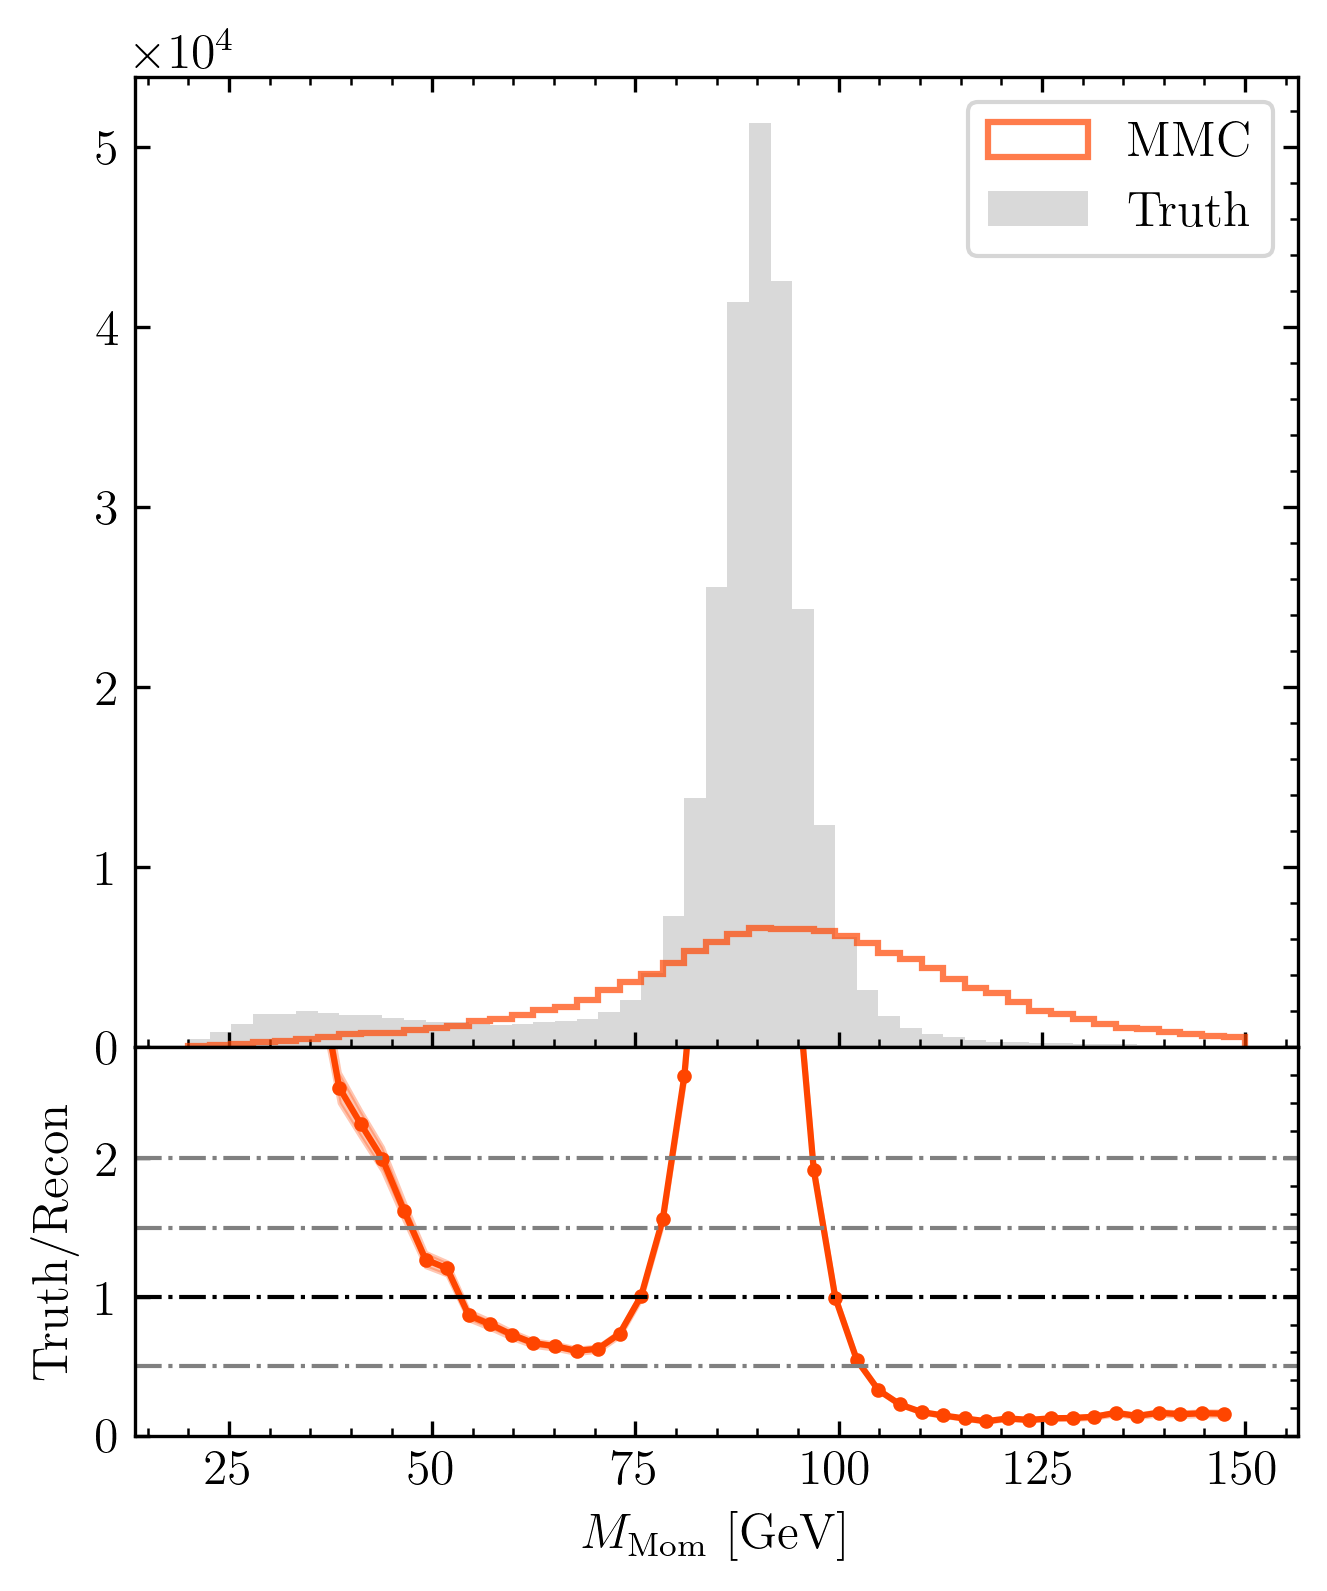
\includegraphics[height=7cm]{figures/mmc}}\hspace{1em}
  \subfloat[生成模型]{
    \label{sfig:Omnil}
    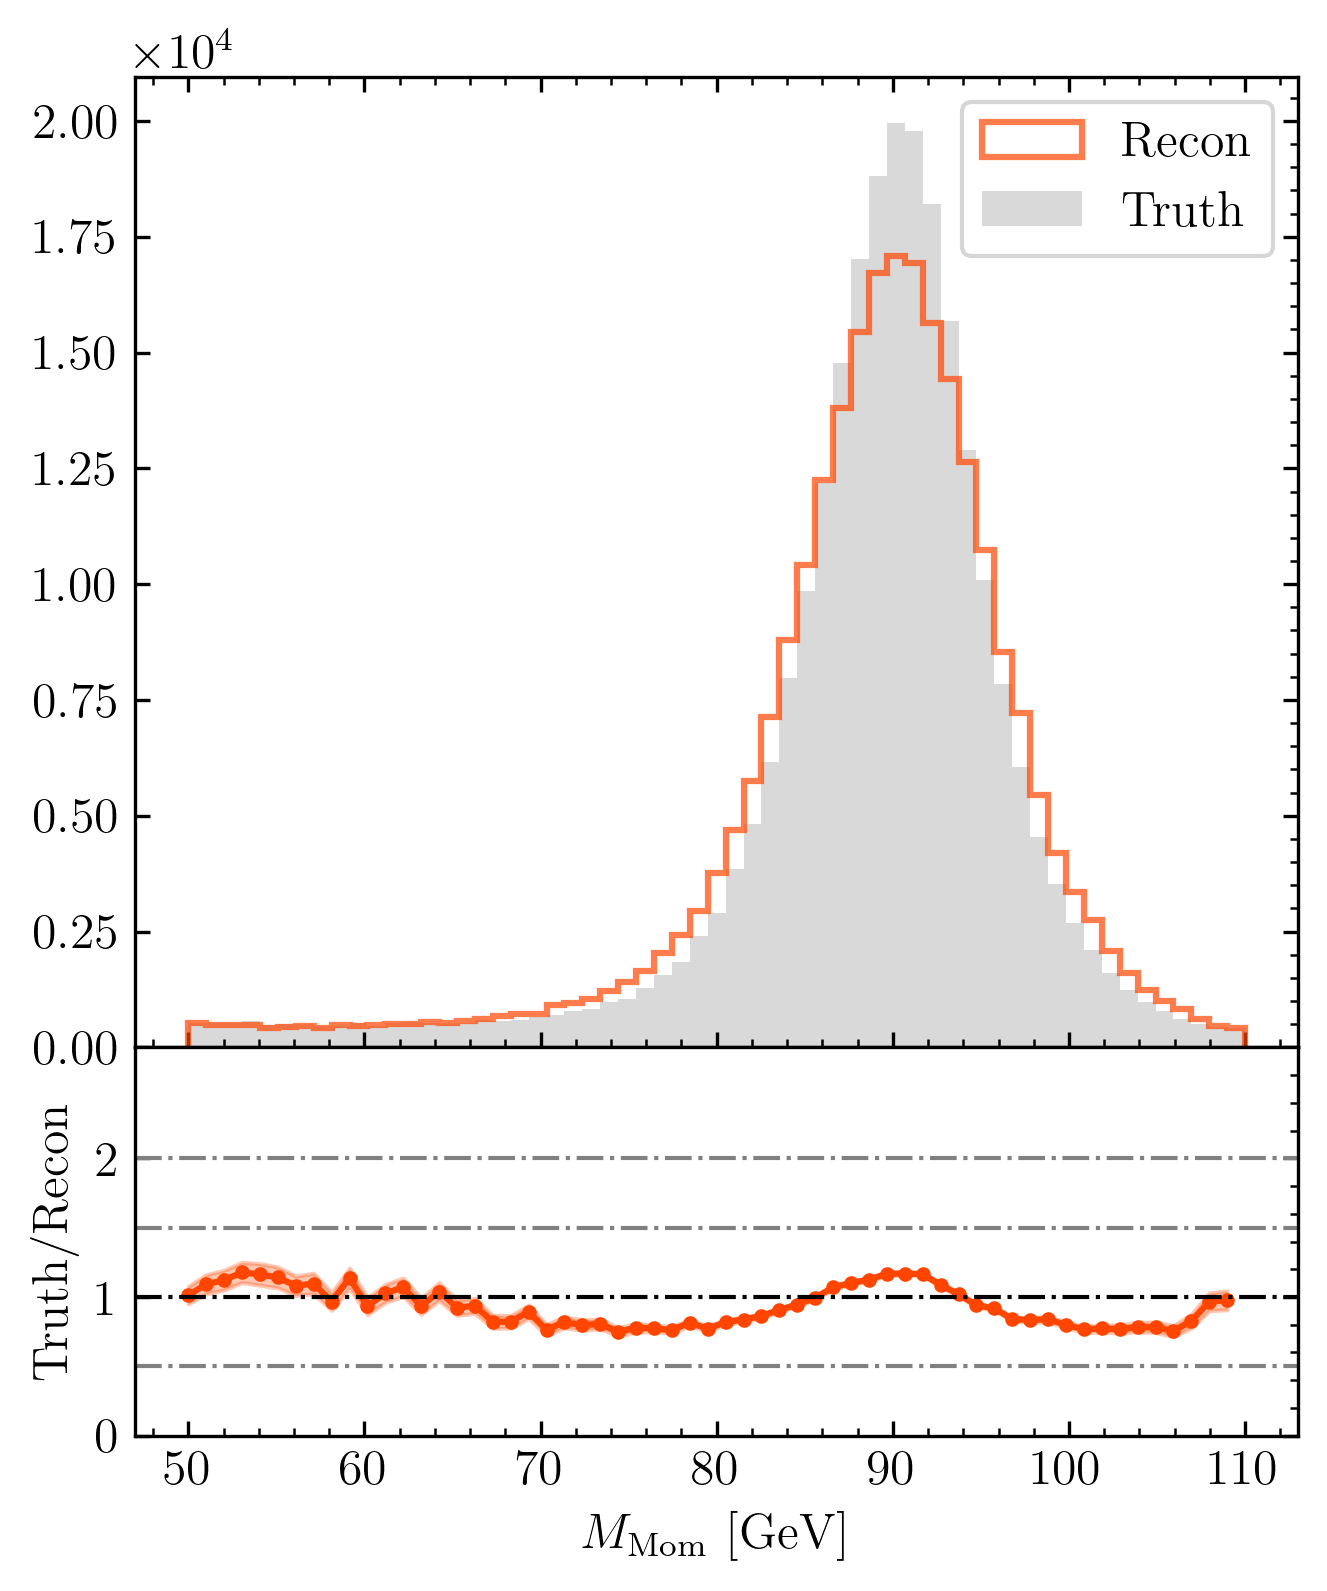
\includegraphics[height=6.97cm]{figures/tautau}}
  \caption{MMC方法与生成模型效果比较}
  \label{fig:MMCcomp}
\end{figure}

由图4-5可以看出，在重建粒子四动量信息上，相比传统的MMC方法，使用生成模型极大地提高了数据重建的准确性。这也是自旋关联矩阵计算结果以及纠缠判断可信的有力佐证。